\documentclass[border={0.1cm 0.1cm}]{standalone}
\usepackage[usenames,dvipsnames]{xcolor}

\usepackage{tikz}
\usetikzlibrary{shapes, arrows, automata, positioning}

\begin{document}
    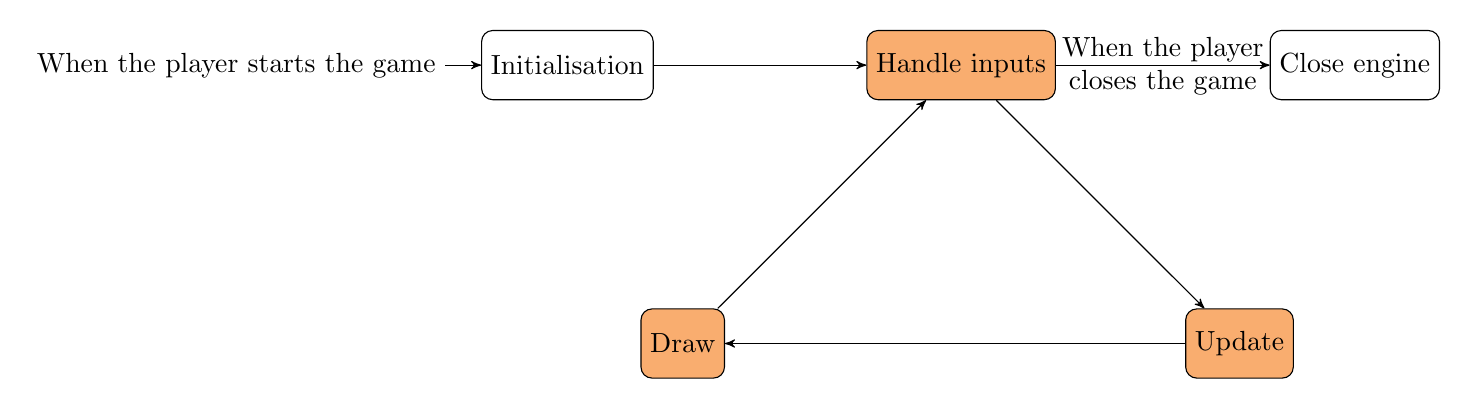
\begin{tikzpicture}[
        ->,>=stealth',
        state/.append style = {
            rectangle,
            rounded corners,
            text centered
        },
        loop/.style = {
            state,
            fill=Apricot
        },
        initial text=When the player starts the game,
        node distance=5cm,
        auto
    ]
        \node [state, initial]  (init)      {Initialisation};
        \node [loop]           (inputs) [right of=init]     {Handle inputs};
        \node [loop]           (update) [below right of=inputs]    {Update};
        \node [loop]           (draw)   [below left of=inputs]  {Draw};
        \node [state]           (end)    [right of=inputs]   {Close engine};

        \path
            (init)      edge            node    {}  (inputs)
            (inputs)    edge            node    {}  (update)
                        edge            node[align=center, above=-0.5cm]    {When the player\\closes the game}  (end)
            (update)    edge            node    {}  (draw)
            (draw)      edge            node    {}  (inputs)
        ;
    \end{tikzpicture}
\end{document}